\documentclass[10pt]{article}
 
\usepackage[margin=1.5cm]{geometry} 
\usepackage{amsmath,amsthm,amssymb}
\usepackage{polski}
\usepackage[utf8]{inputenc}
\usepackage{siunitx}
\usepackage{graphicx}
\usepackage{comment}
\usepackage[font=scriptsize]{caption}
\usepackage{subcaption} 
\usepackage{array}
\usepackage{hyperref}
\usepackage[section]{placeins}

\newcolumntype{C}[1]{>{\centering\let\newline\\\arraybackslash\hspace{0pt}}m{#1}}

\newenvironment{theorem}[2][Twierdzenie]{\begin{trivlist}
\item[\hskip \labelsep {\bfseries #1}\hskip \labelsep {\bfseries #2.}]}{\end{trivlist}}
\newenvironment{question}[2][Pytanie]{\begin{trivlist}
\item[\hskip \labelsep {\bfseries #1}\hskip \labelsep {\bfseries #2.}]}{\end{trivlist}}
\newenvironment{hypothesis}[2][Hipoteza]{\begin{trivlist}
\item[\hskip \labelsep {\bfseries #1}\hskip \labelsep {\bfseries #2.}]}{\end{trivlist}}
\newenvironment{lemma}[2][Lemat]{\begin{trivlist}
\item[\hskip \labelsep {\bfseries #1}\hskip \labelsep {\bfseries #2.}]}{\end{trivlist}}
\newenvironment{exercise}[2][Ćwiczenie]{\begin{trivlist}
\item[\hskip \labelsep {\bfseries #1}\hskip \labelsep {\bfseries #2.}]}{\end{trivlist}}
\newenvironment{reflection}[2][Uwaga]{\begin{trivlist}
\item[\hskip \labelsep {\bfseries #1}\hskip \labelsep {\bfseries #2.}]}{\end{trivlist}}
\newenvironment{proposition}[2][Założenie]{\begin{trivlist}
\item[\hskip \labelsep {\bfseries #1}\hskip \labelsep {\bfseries #2.}]}{\end{trivlist}}
\newenvironment{corollary}[2][Wniosek]{\begin{trivlist}
\item[\hskip \labelsep {\bfseries #1}\hskip \labelsep {\bfseries #2.}]}{\end{trivlist}}
\newcommand{\expnumber}[2]{{#1}\mathrm{e}{#2}}

\begin{document}
\[\title{Aproksymacja średniokwadratowa dyskretna}
\author{Grams, Stanisław\\Jezierski, Maciej\\Korczakowski, Juliusz\\ MFI UG\\Algorytmy Numeryczne}

\maketitle
\section {Implementacja}
Program \textit{„approximations”} został napisany w języku C++ a wyniki działania programu zapisywane są do poszczególnych plików \textit{*.csv}.
\subsection{Zaimplementowane oraz użyte algorytmy}
\begin{itemize}
	\item (\textbf{G}): Algorytm Gaussa z częściowym wyborem elementu
	\item (\textbf{G\_SPARSE}): Algorytm Gaussa z częściowym wyborem elementu i optymalizacją dla macierzy rzadkich 
	\item (\textbf{GS\_1E10}): Algorytm Gaussa-Seidela (precyzja \num{1e-10}, struktura macierzy tablicowa)
	\item (\textbf{GS\_EIGEN}): Algorytm Gaussa-Seidela z implementacją dla biblioteki $Eigen3$ (precyzja \num{1e-10})
	\footnote{\url{http://komi.web.elte.hu/elektronikus/src/p184-koester.pdf}}
	\item (\textbf{LU\_EIGEN}): Algorytm SparseLU pochodzący z biblioteki $Eigen3$
	\footnote{\url{https://eigen.tuxfamily.org/dox/classEigen_1_1SparseLU.html}}
\end{itemize}
W celu obsługi metod \textbf{GS\_EIGEN} oraz \textbf{LU\_EIGEN} oparteych o bibliotekę $Eigen3$ należało w dodatku do\\
zadania nr 3 doimplementować klasy \textit{SparseMatrix} oraz \textit{SparseGenerator} pozwalające na wydajne operacje na nowych typach.\\
Testy zostały wykonane dla ilości agentów równej $N = 3 .. 60$.\\
\textbf{Przypomnienie:} rząd macierzy można wyznaczyć ze wzoru $A = \frac{(N+1) * (N+2)}{2}$ 
\section{Analiza wyników}

\begin{figure}[h]
\centering
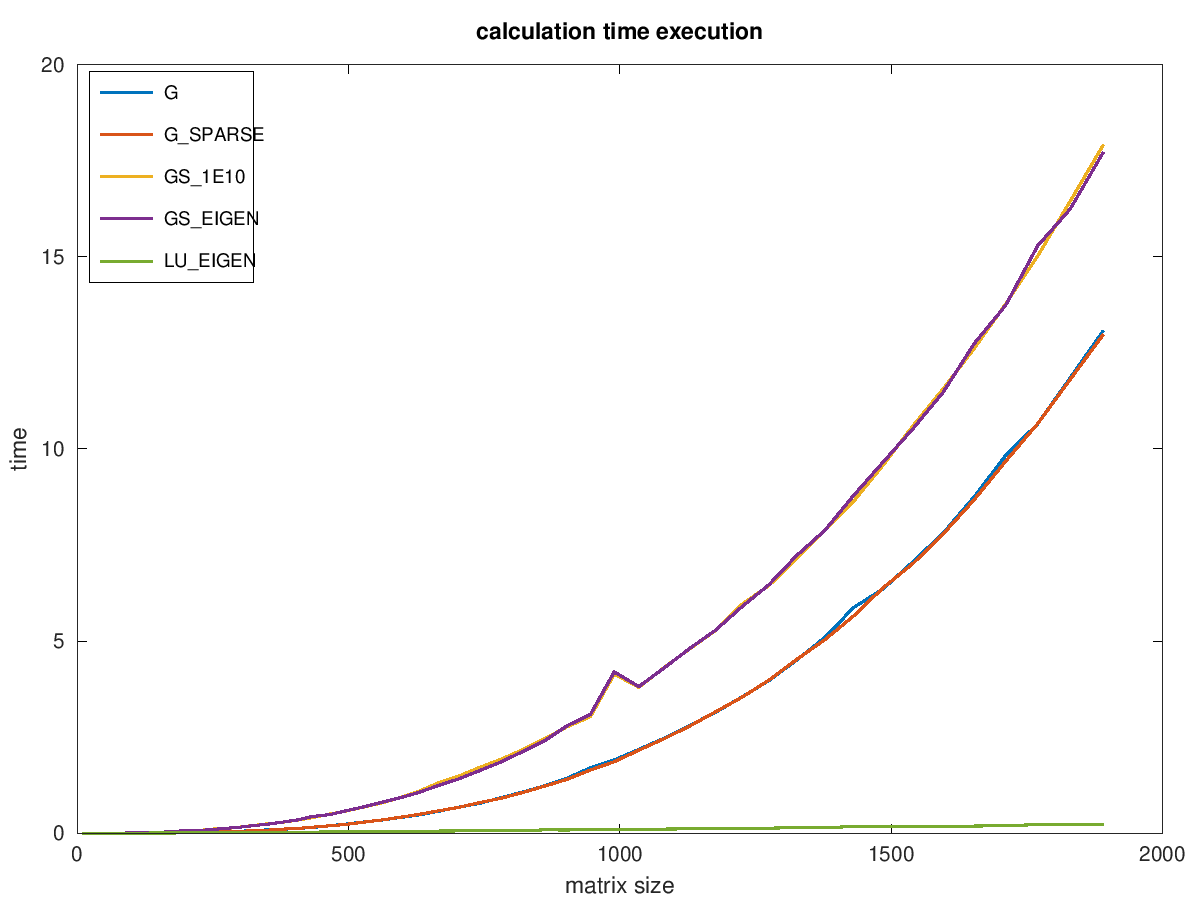
\includegraphics[scale=0.40]{plots/01_calc_time_execution_all_methods.png}
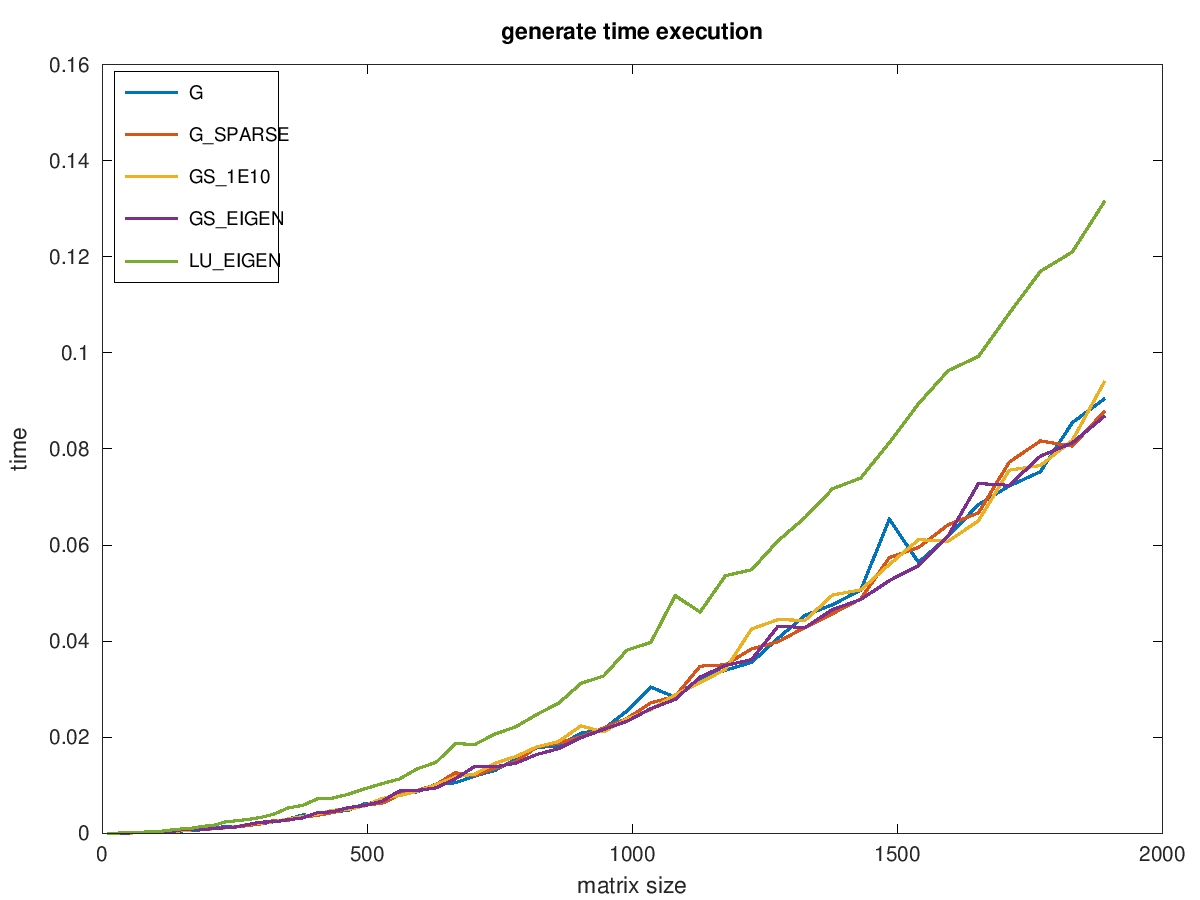
\includegraphics[scale=0.40]{plots/02_gen_time_execution_all_methods.png}
\end{figure}

\begin{figure}[h]
\centering
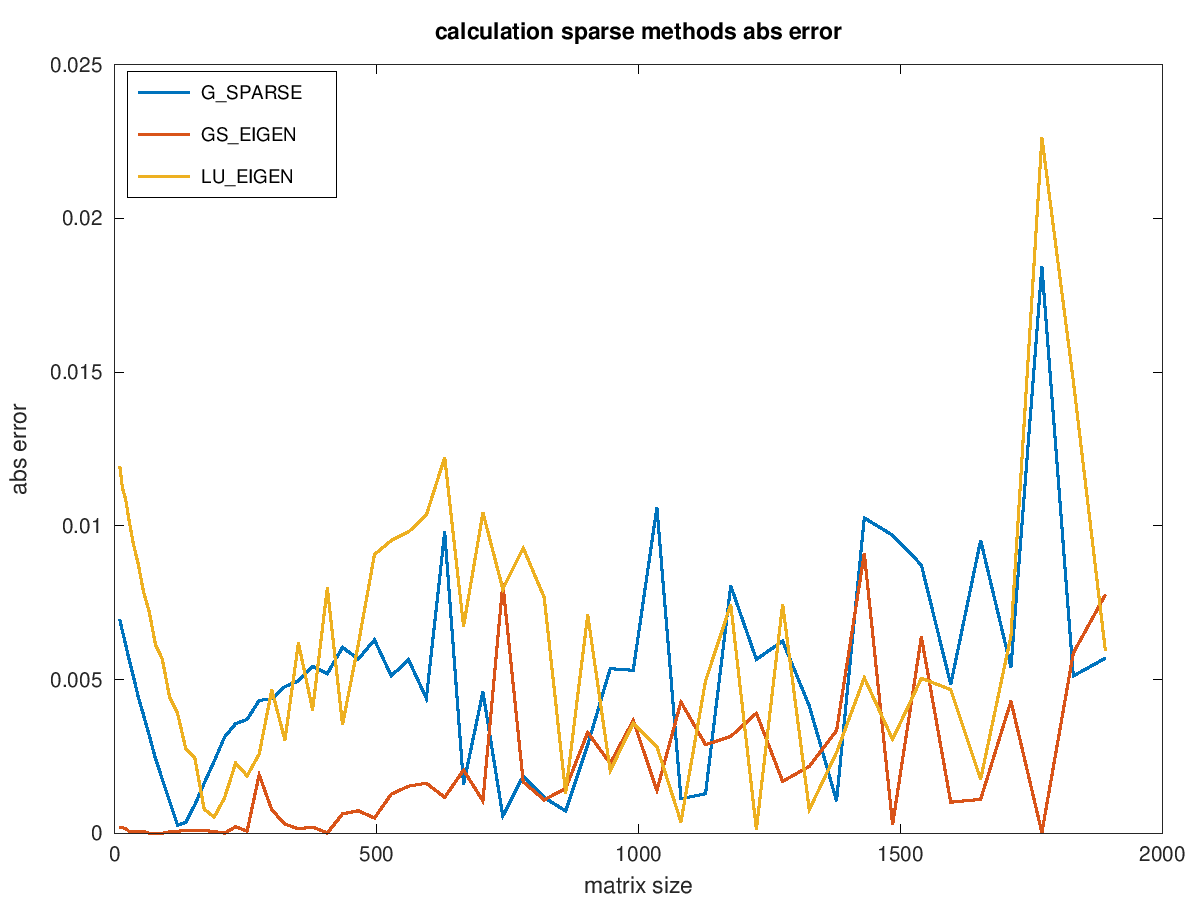
\includegraphics[scale=0.45]{plots/03_calc_abs_error_sparse_methods.png}
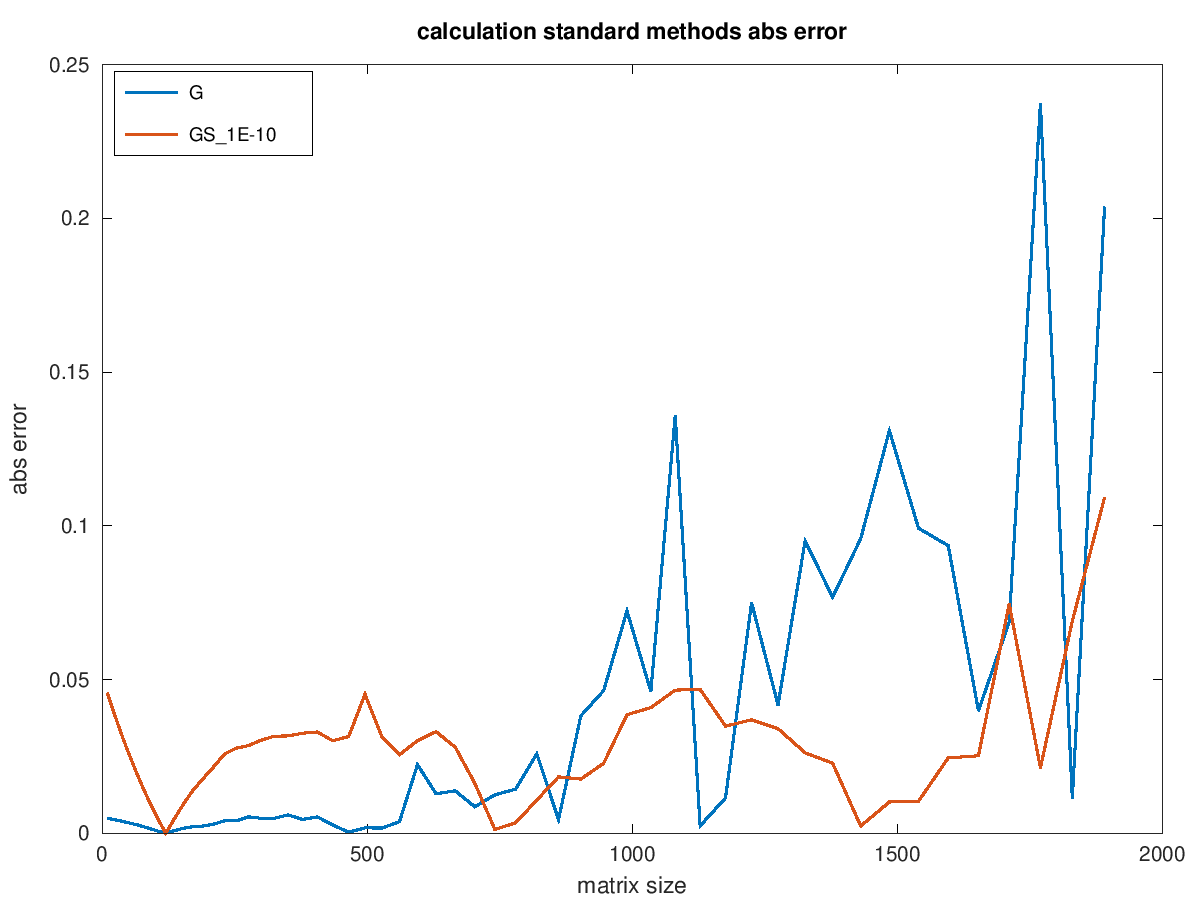
\includegraphics[scale=0.45]{plots/04_calc_abs_error_standard_methods.png}
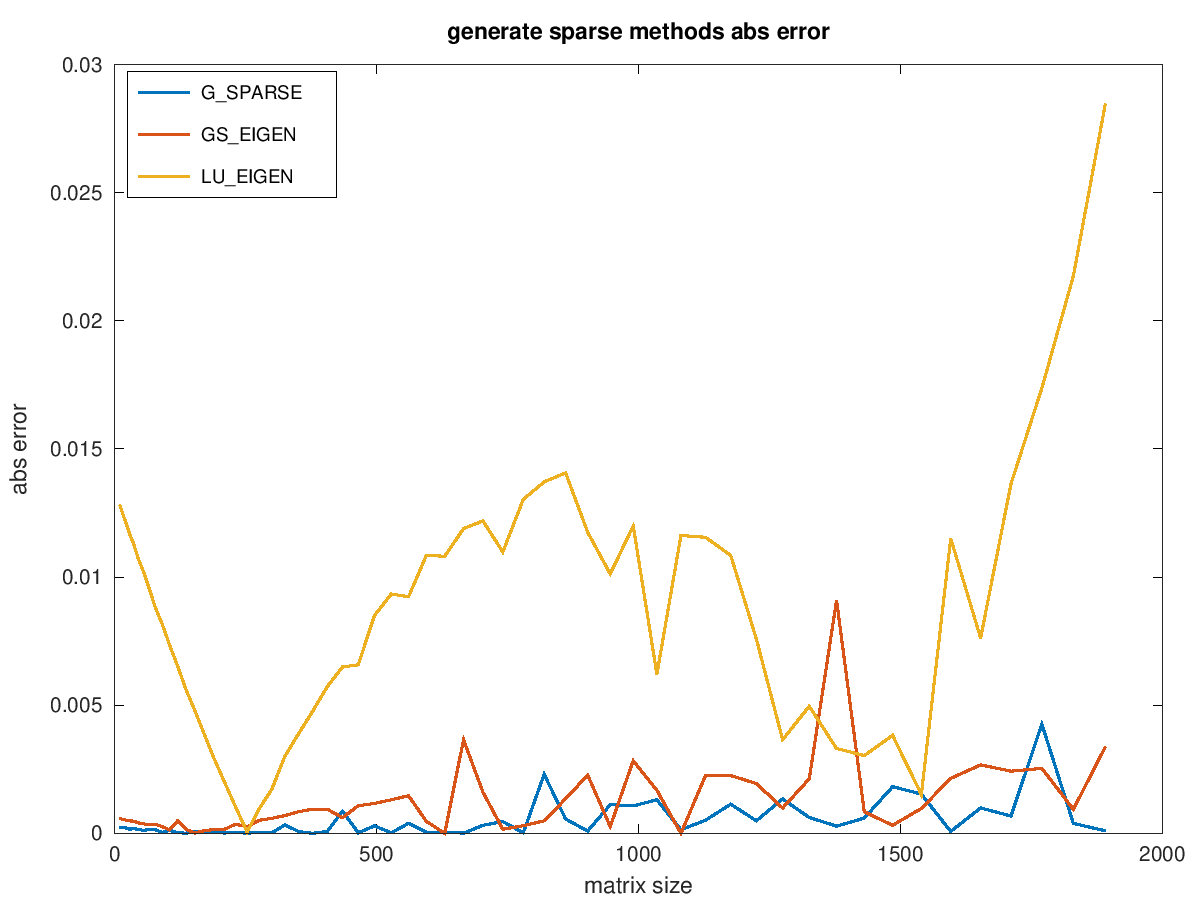
\includegraphics[scale=0.45]{plots/05_gen_abs_error_sparse_methods.png}
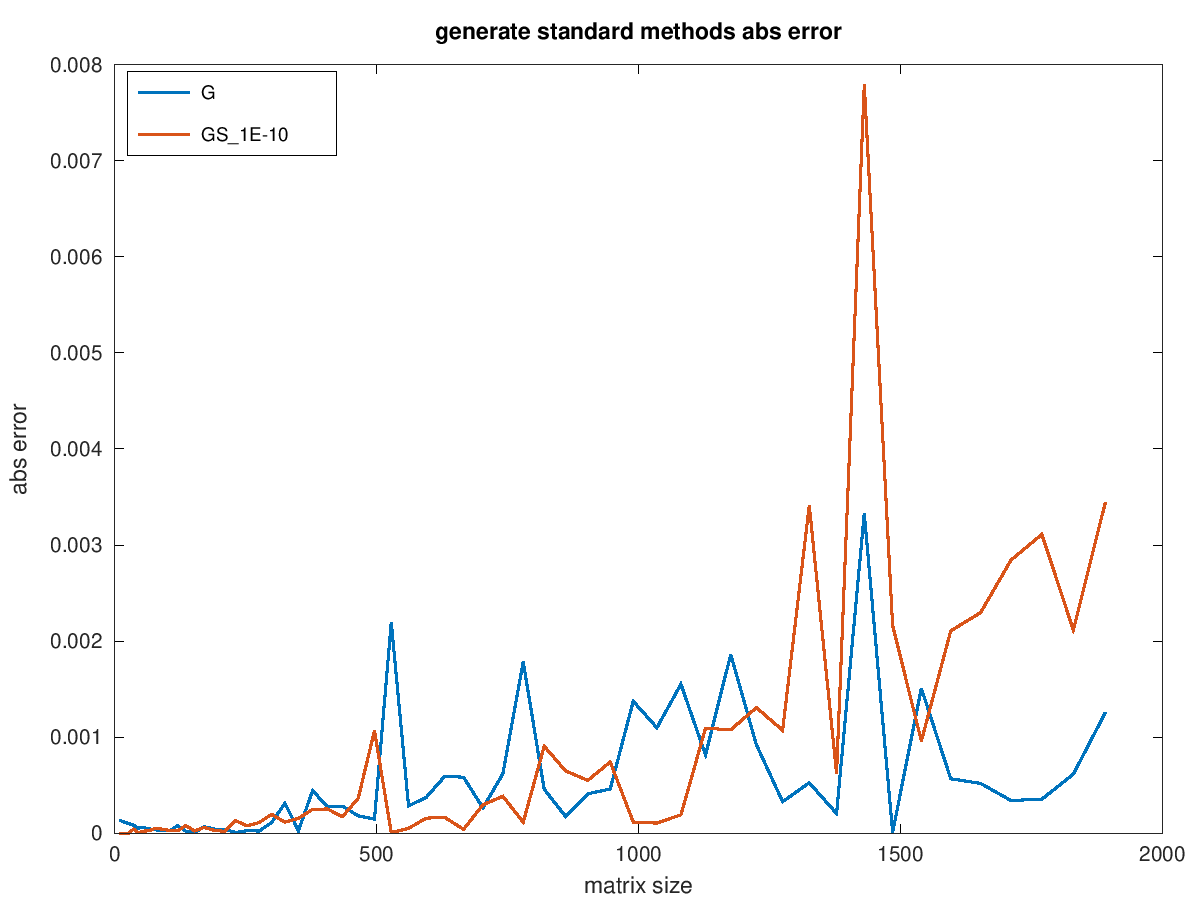
\includegraphics[scale=0.45]{plots/06_gen_abs_error_standard_methods.png}
\end{figure}

\section{Aproksymacja}
\begin{figure}[h]
	\centering
	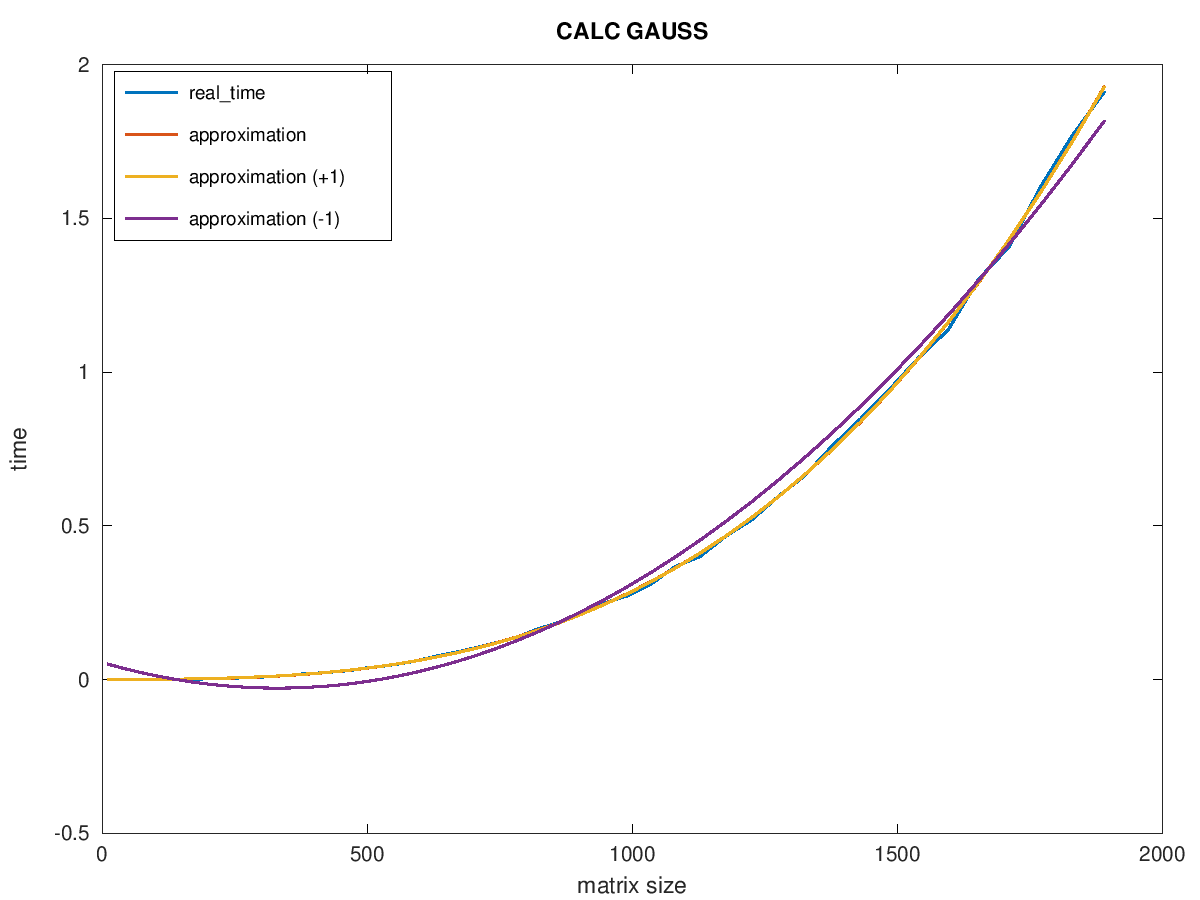
\includegraphics[scale=0.45]{plots/07_calc_gauss_plus_minus_time.png}
	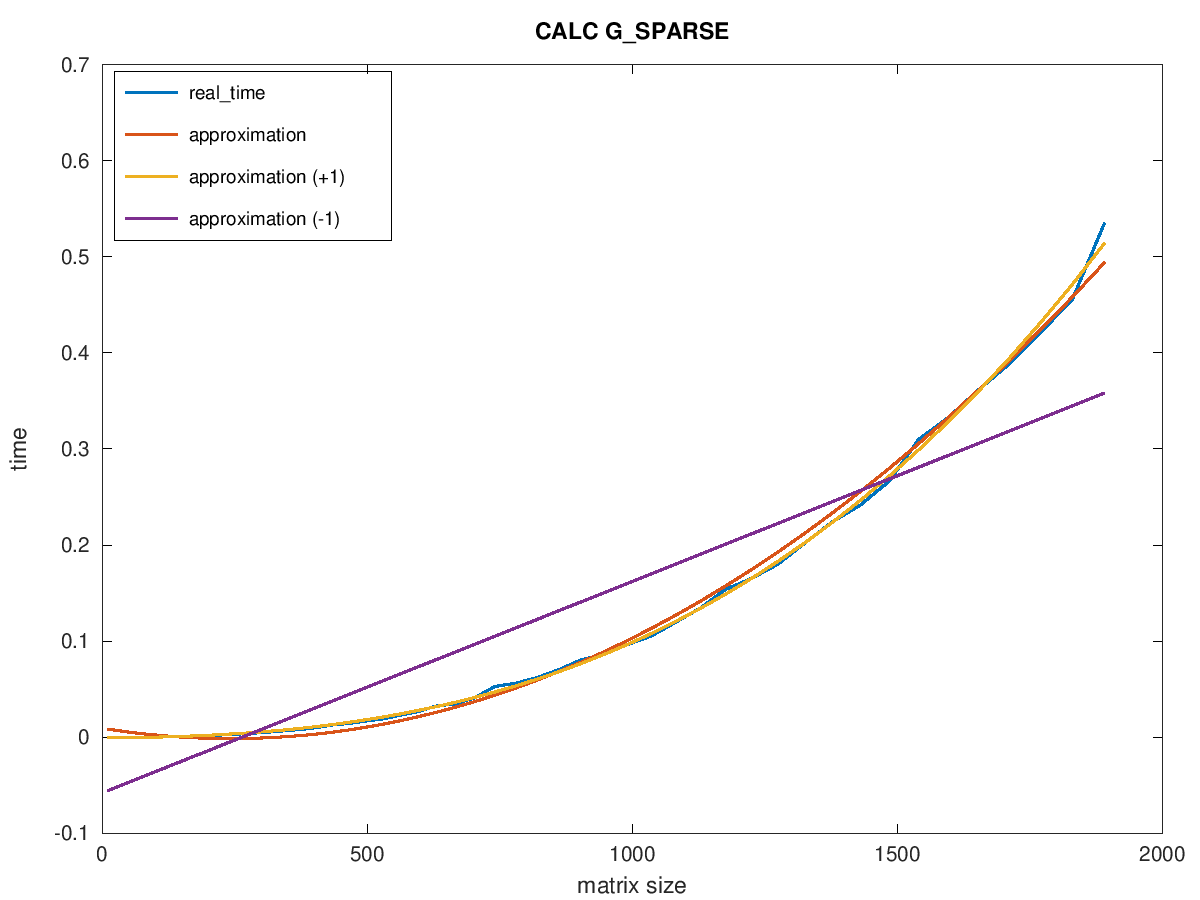
\includegraphics[scale=0.45]{plots/09_calc_gauss_sparse_plus_minus_time.png}
\end{figure}
\begin{figure}[h]
	\centering
	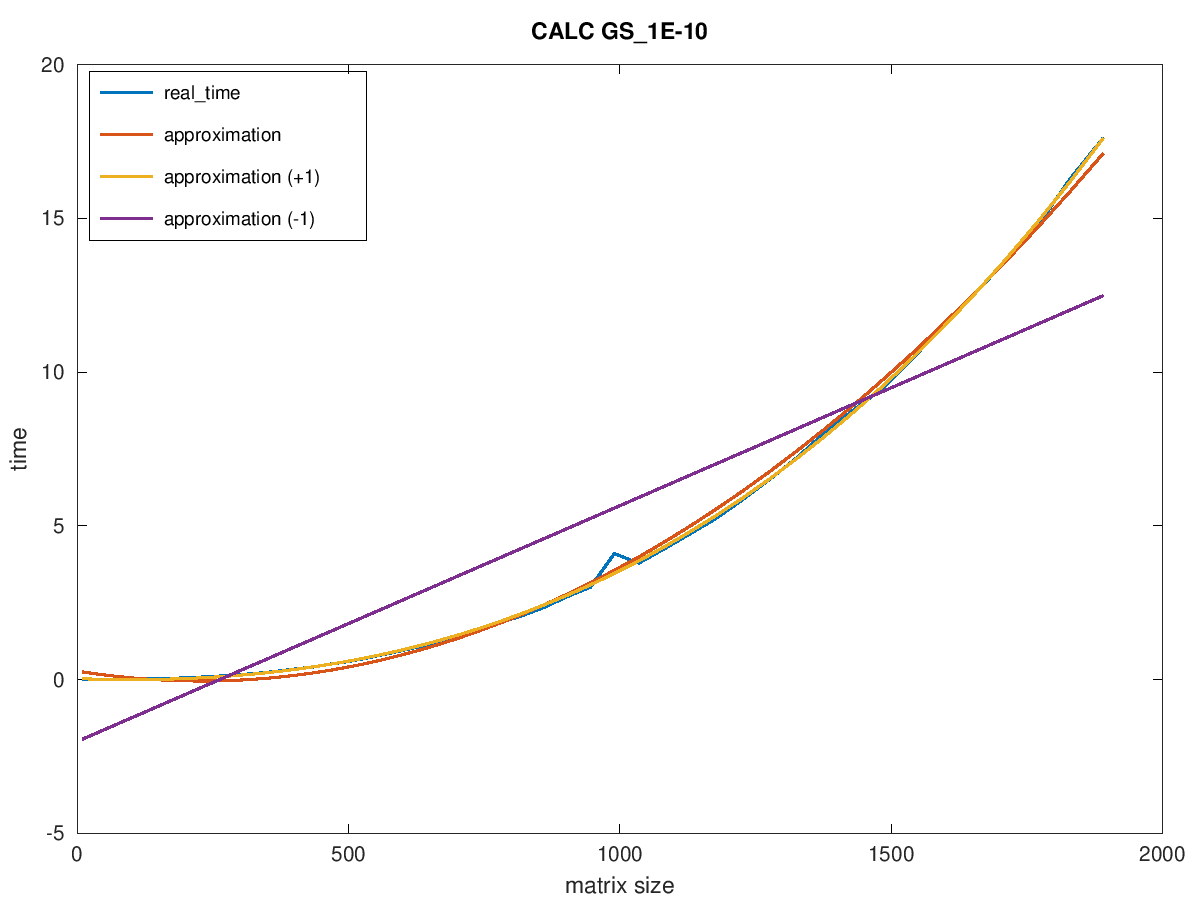
\includegraphics[scale=0.3]{plots/11_calc_gauss_1e10_plus_minus_time.png}
	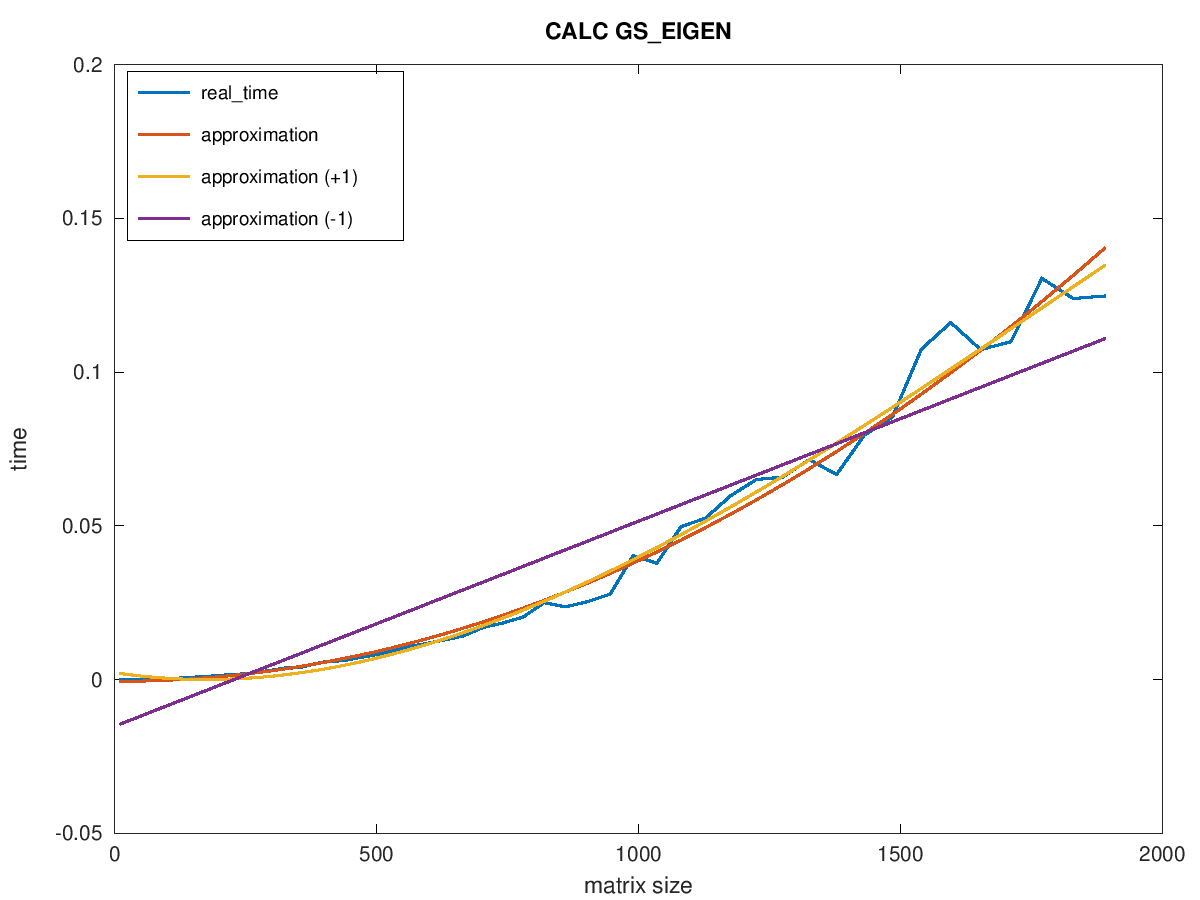
\includegraphics[scale=0.3]{plots/13_calc_gauss_eigen_plus_minus_time.png}
	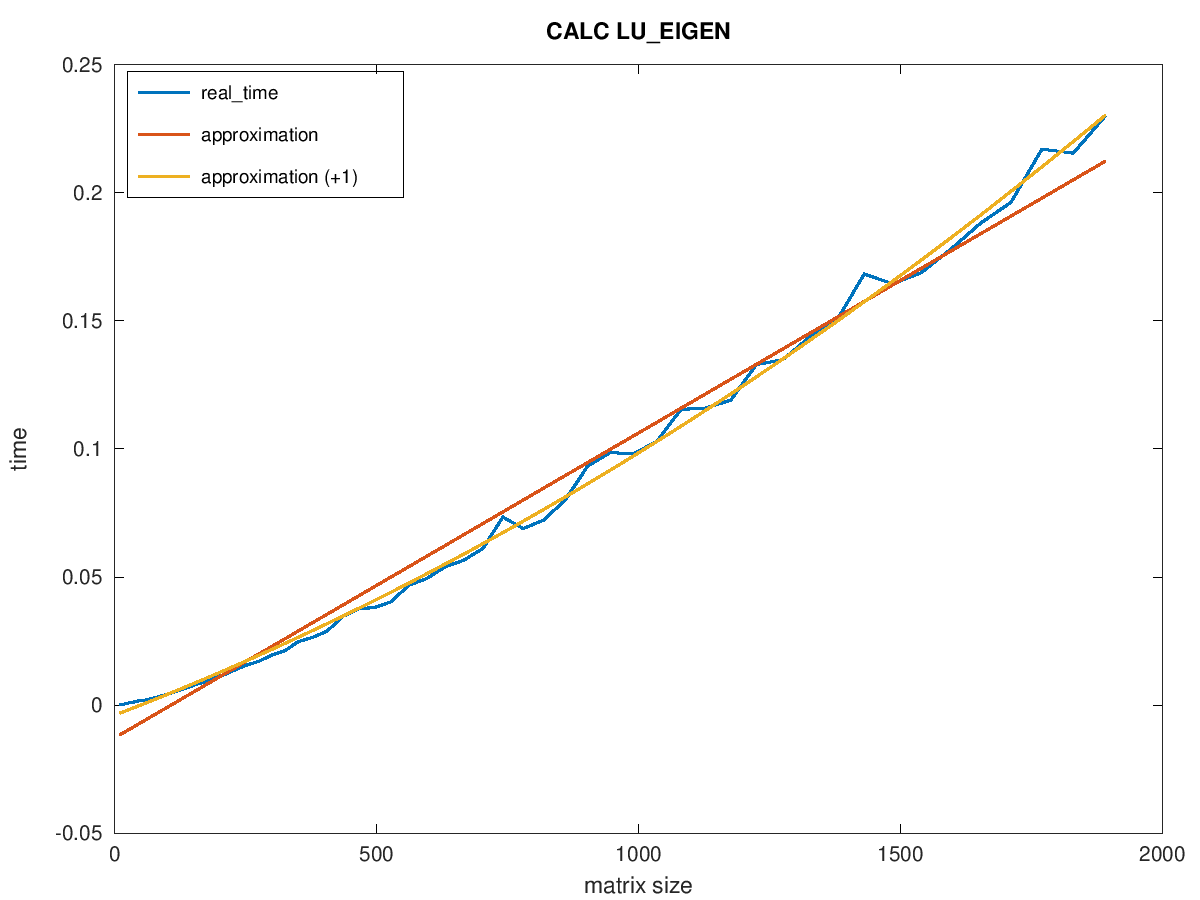
\includegraphics[scale=0.3]{plots/15_calc_lu_eigen_plus_minus_time.png}
\end{figure}
\subsection{Wyliczone współczynniki wielomianów}
\begin{itemize}
	\item Rozwiązywanie układu równań:
	\begin{enumerate}
		\item (\textbf{G}): $f(x) = \expnumber{1.88345}{-9} x^3 + \expnumber{5.25579}{-8} x^2 + (\expnumber{-1.30456}{-5}) x^1 + 0.00124971$
		\item (\textbf{G\_SPARSE}): $f(x) = \expnumber{1.82546}{-7} x^2 + (\expnumber{-8.8859}{-5}) x^1 + 0.00941105$
		\item (\textbf{GS\_1E10}): $f(x) = \expnumber{6.21178}{-6} x^2 + (-0.00284503) x^1 + 0.279666$
		\item (\textbf{GS\_EIGEN}): $f(x) = \expnumber{1.25348}{-7} x^2 + \expnumber{6.14431}{-6} x^1 - 0.00112571$
		\item (\textbf{LU\_EIGEN}): $f(x) = 0.000119035 x^1 - 0.0127681$
	\end{enumerate}
	\item Generowanie macierzy:
	\begin{enumerate}
		\item (\textbf{G}): $f(x) = \expnumber{-2.06199}{-12} x^3 + \expnumber{2.9385}{-8} x^2 + \expnumber{-2.30313}{-6} x^1 + 0.000161398$
		\item (\textbf{G\_SPARSE}): $f(x) = \expnumber{2.54238}{-8} x^2 + (\expnumber{-1.99597}{-6}) x^1 - 0.000262153$
		\item (\textbf{GS\_1E10}): $f(x) = \expnumber{2.4649}{-8} x^2 + (\expnumber{-1.68417}{-7}) x^1 + \expnumber{5.40007}{-6}$
		\item (\textbf{GS\_EIGEN}): $f(x) = \expnumber{3.39916}{-8} x^2 + \expnumber{5.10909}{-8} x^1 - 0.000618658$
		\item (\textbf{LU\_EIGEN}): $f(x) = \expnumber{6.26423}{-5} x^1 - 0.0134335$
	\end{enumerate}
\end{itemize}
\subsection{Poprawność wyników aproksymacji – średnie błędy bezwzględne}
\begin{center}
		\begin{tabular}{|C{2.5cm}| C{5cm}|C{5cm}|}
			\hline
			\textbf{} & \textbf{Obliczanie} & \textbf{Generowanie} \\ \hline
			{G} & 0.116641068509220541 & 0.006139134153799684  \\ \hline
			{G\_SPARSE} & 0.061993311882769679 & 0.006427472787361275 \\  \hline
			{GS\_1E10} & 1.467795323159247101 & 0.011466237689022329 \\  \hline
			{GS\_EIGEN} & 0.019821774223782174 & 0.013693956132461119\\ \hline
			{LU\_EIGEN} & 0.056598547270937556 & 0.076729386139618563\\ \hline
		\end{tabular}
\end{center}
\begin{corollary}{1}
	Uzyskane wyniki znajdują się w granicy tolerancji błędu dla funkcji aproksymującej opartej o aproksymacje średniokwadratową dyskretną.

\end{corollary}

\section{Ekstrapolacja}
\subsection{Ekstrapolacja czasu obliczeń dla układu o rozmiarze rzędu $100 000$}
\begin{center}
	\begin{tabular}{|C{2.5cm}|C{5cm}|}
		\hline
		\textbf{} & \textbf{Wyliczony czas [s]}\\ \hline
		{G} & 2087048.540863713948056102 \\ \hline
		{G\_SPARSE} & 1842.864744169787172723 \\  \hline
		{GS\_1E10} & 67836.170996347194886766 \\  \hline
		{GS\_EIGEN} & 1297.890374618339365043 \\ \hline
		{LU\_EIGEN} & 12.933910601128554063 \\ \hline
	\end{tabular}
\end{center}
	
\section{Próba obliczenia układu o rozmiarze rzędu $100 000$ i klasa SparseMatrix}
	Jako najszybszą metodę uznaliśmy \textbf{LU\_EIGEN} i tą metodą wykonaliśmy test dla macierzy rzędu \num{100128} (\num{446} agentów).
	Uzyskany czas wynosi \textbf{$58.611972999999998990$} i jest około 4.9x gorszy od aproksymowanego.
	Metody oparte o bibliotekę $Eigen3$ odznaczają się również znacznie niższym zużyciem pamięci operacyjnej.

\section{Podział pracy}
\begin{center}
	\begin{tabular}{| p{6cm} | p{6cm} | p{6cm} |}
		\hline
		\textbf{Stanisław Grams} & \textbf{Juliusz Korczakowski} & \textbf{Maciej Jezierski} \\ \hline
		Implementacja algorytmu Gaussa-Seidela & Implementacja klasy Approximation & Przygotowanie sprawozdania  \\ \hline
		Implementacja klasy SparseMatrix oraz SparseGenerator w oparciu o $Eigen3$ & Przygotowanie wykresów oraz tabel & Agregacja uzyskanych wyników \\ \hline
		Implementacja wywołania poszczególnych prób ($main.cc$) & Uruchomienie prób i testowanie & Praca nad strukturą projektu\\ \hline
	\end{tabular}
\end{center}
\]
\end{document}